\section{Dataset}
\label{dataset}

The raw consultation dialogue data comes from the doctor and patient Q\&A 
forum on the online medical website ``Chunyu Doctors''\footnote{https://www.chunyuyisheng.com.}. 
The forum is divided into 14 top-level departments, 
each of which consisting of several second-level departments, 
accompanied by the classification of diseases. 
Each Q\&A consists of several rounds of a dialogue between a patient and a doctor. In order to understand as much as possible the semantic context of different disease situations, this study crawls all the classical Q\&A dialogues corresponding to the departments of top-level and second-level, reaching more than 100,000 Q\&A pairs, named D-P QA.

\begin{figure}[h]
\centering
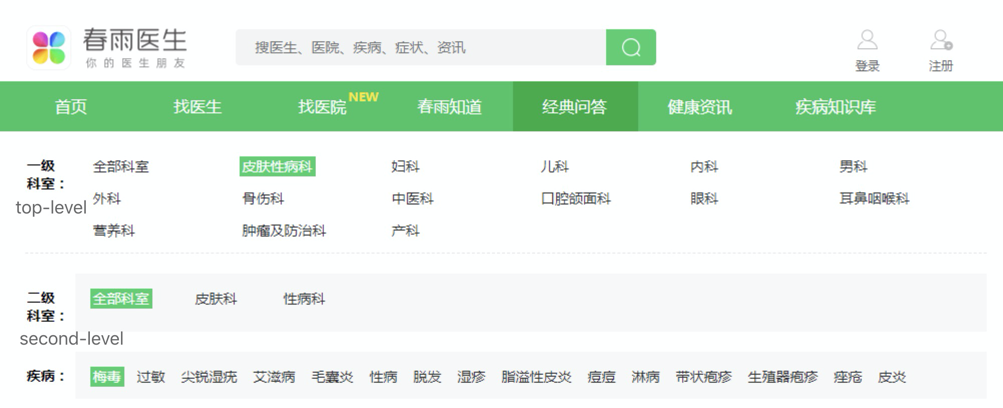
\includegraphics[scale=0.3]{2.png}
\caption{The original forum in the website.}
\label{fig:figure1}
\end{figure}

During data crawling, to circumvent the blocking of IPs by the web server, 
we set up a proxy pool. 
Setting up the proxy pool can be divided into three steps, as shown in Figure \ref{fig:figure2} : 
\begin{itemize}
\item[(1)]Acquisition module. The purpose is in the proxy web site to grab the proxy IP. The form of the proxy is IP plus port. Try to get proxies from different sources and try to choose high hiding proxies. 
\item[(2)]Detection module. We identify the state of each proxy and set the score identifier for it, with an initial value of 10. The lower the score, the less available it is. The detection process is as follows. Test once. If the proxy is available, the score can be set to 100. If the proxy is not available, subtract 1 point from the score and remove the proxy when the score is reduced to a threshold value, such as 0. Finally, the available proxies are stored in the database.
\item[(3)]Interface module. We provide a Web API interface so that we can access the available proxies by accessing the interface. In addition, if a certain proxy needs to be returned randomly, it is necessary to obtain the proxy with the highest score in the ranking.
\end{itemize}

\begin{figure}[th]
\centering
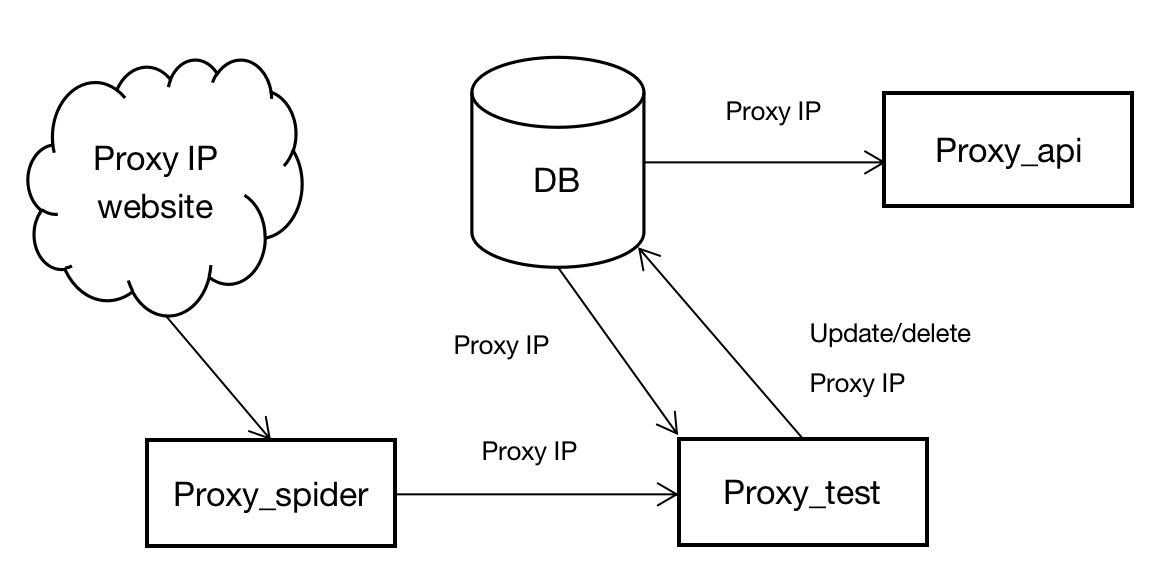
\includegraphics[scale=0.35]{1.png}
\caption{The process of setting up a proxy pool.}
\label{fig:figure2}
\end{figure}

Traditional Chinese text processing usually needs to remove stop words to reduce text redundancy. However, we do not design the operation of removing the stop words. The reason lies in the particularity of the question. Stop words could be important parts of the question. In addition, we delete Q$\&$A with less than one round of conversations and conversations that are considered invalid, because there are no clarifications in them but they can be a part of negative examples.
We also cut out conversations without substantive contents, such as those with only greetings between speakers but without consultation. And finally we remove redundant spaces and perform field de duplication.

We randomly select 1000 sentences of what the expert says in all the processed conversations as the test set and the rest as the training set. Then manually mark the types of 1000 sentences. Label the front of each sentence. For examples, in \tabref{tab:example1}, ``Have you ever had an allergy check?'' is a clarification question, classified as ``Q''; and ``This is a seasonal allergy. You'd better have it checked.'' is an answer, classified as ``A''. Finally, we get a labelled dataset, in which each dialogue has at least two rounds, with an average of five rounds. Each dialogue has at least one clarification question.
The complete dataset, including the labelled test set, can be downloaded from \url{http://anonymized.for.blind.review}.
